\documentclass[a4paper,12pt]{article}
\usepackage[utf8]{inputenc}
\usepackage{graphicx} % Para inserir imagens
\usepackage{listings}
\usepackage{color}

% Configuração para mostrar código fonte
\lstset{
  basicstyle=\ttfamily\footnotesize,
  keywordstyle=\color{blue},
  commentstyle=\color{gray},
  stringstyle=\color{red},
  numbers=left,
  numberstyle=\tiny\color{gray},
  stepnumber=1,
  numbersep=5pt,
  backgroundcolor=\color{white},
  showspaces=false,
  showstringspaces=false,
  showtabs=false,
  tabsize=2,
  captionpos=b,
  breaklines=true,
  breakatwhitespace=false,
  title=\lstname,
  escapeinside={\%*}{*)},
  morekeywords={*,...},
}

\title{Simulação de Inicialização de LEDs em Arduino}
\author{João Daniel da Silva}
\date{\today}

\begin{document}

\maketitle

\section{Introdução}
Este relatório apresenta uma aplicação básica usando a plataforma Arduino para simular um sistema de semáforo com três LEDs: verde, amarelo e vermelho. A aplicação utiliza a plataforma online de simulação Tinkercad, onde o código é testado para garantir seu funcionamento correto. O código consiste em uma sequência de acionamento de LEDs para simular um semáforo típico.

\section{Configuração do Circuito}
A simulação é configurada da seguinte forma:
\begin{itemize}
  \item Um LED vermelho conectado ao pino 0 do Arduino.
  \item Um LED amarelo conectado ao pino 1 do Arduino.
  \item Um LED verde conectado ao pino 2 do Arduino.
\end{itemize}

Segue uma imagem do circuito usado na simulação:

\begin{figure}[h]
  \centering
  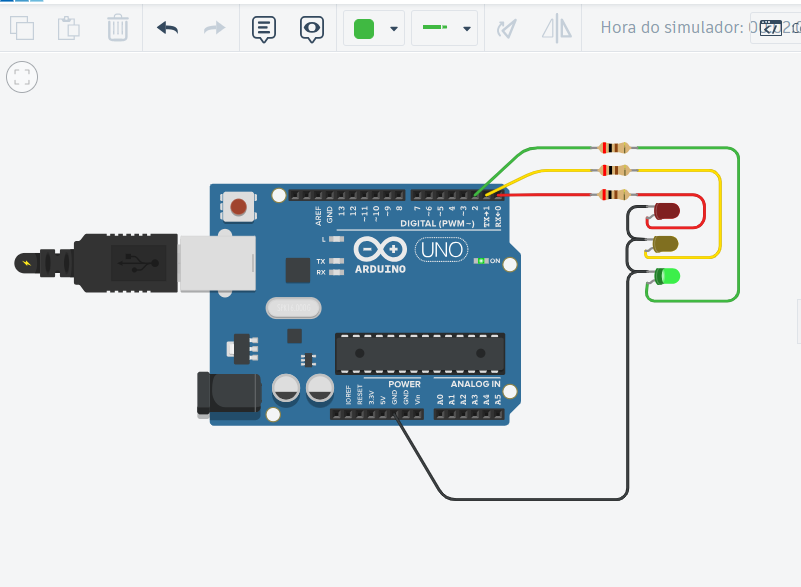
\includegraphics[width=0.8\textwidth]{Captura de tela 2024-05-08 195051.png} % Nome do arquivo da imagem
  \caption{Imagem do circuito ou simulação}
\end{figure}

\section{Código Fonte}
A seguir está o código usado para controlar o sistema de semáforo:

\begin{lstlisting}[language=C]
int led_red = 0; // LED vermelho no pino 0
int led_yellow = 1; // LED amarelo no pino 1
int led_green = 2; // LED verde no pino 2

void setup() {
  pinMode(led_red, OUTPUT);
  pinMode(led_yellow, OUTPUT);
  pinMode(led_green, OUTPUT);
}

void loop() {
  // Ativar o LED verde e desativar os outros
  digitalWrite(led_red, LOW); 
  digitalWrite(led_yellow, LOW);
  digitalWrite(led_green, HIGH);
  delay(2000);    // Aguardar 2 segundos
  
  // Ativar o LED amarelo e desativar os outros
  digitalWrite(led_red, LOW);   
  digitalWrite(led_yellow, HIGH);
  digitalWrite(led_green, LOW);
  delay(1000);   // Aguardar 1 segundo
  
  // Ativar o LED vermelho e desativar os outros
  digitalWrite(led_red, HIGH);  
  digitalWrite(led_yellow, LOW);
  digitalWrite(led_green, LOW);
  delay(3000);  // Aguardar 3 segundos        
}
\end{lstlisting}

\section{Funcionamento}
O código controla a sequência de LEDs para simular o comportamento de um semáforo. O LED verde acende por 2 segundos, seguido do LED amarelo por 1 segundo e depois do LED vermelho por 3 segundos. Esta sequência é repetida continuamente no loop principal.

\section{Plataforma de Simulação}
Para testar o código, utilizamos a plataforma de simulação Tinkercad. Através dela, é possível criar circuitos virtuais e testar o código em um ambiente seguro. As simulações permitem entender o comportamento do semáforo antes de implementar um circuito físico.

\section{Conclusão}
Este relatório apresentou uma aplicação básica de Arduino para controlar LEDs como um sistema de semáforo. Através do uso de uma plataforma online como o Tinkercad, a simulação foi testada e validada. Esta aplicação serve como uma introdução ao mundo do Arduino e suas aplicações práticas. Futuras melhorias podem incluir a adição de sensores ou controle remoto para um semáforo mais avançado.

\end{document}
